\documentclass[a4paper,12pt]{book} % nie: report!


% pakiety
\usepackage{polski} % lepiej to zamiast babel!
\usepackage[utf8]{inputenc} % w razie kłopotów spróbować: \usepackage[utf8x]{inputenc}
\usepackage{fancyhdr} % nagłówki i stopki
\usepackage{indentfirst} % WAŻNE, MA BYĆ!
\usepackage{lipsum}
\usepackage[pdftex]{graphicx} % to do wstawiania rysunków
\usepackage{amsmath} % to do dodatkowych symboli, przydatne
\usepackage[pdftex,
            left=1in,right=1in,
            top=1in,bottom=1in]{geometry} % marginsy
\usepackage{amssymb} % to też do dodatkowych symboli, też przydatne
\usepackage{pdfpages} % żeby wstawić stronę tytułową
% jesli potrzeb, można oczywiście wstawić inne pakiety i swoje definicje...
\usepackage{graphicx}
\graphicspath{{./pictures}}
\usepackage{import}
\usepackage{svg}

\usepackage{pgfplots}

\usepackage{xstring}
\usepackage{tikz}
\usepackage{listofitems}
\usepackage{etoolbox}
\usetikzlibrary{arrows.meta, fit, positioning} % for arrow size
\usepackage[outline]{contour} % glow around text
\contourlength{1.4pt}
\tikzstyle{mynode}=[thick,draw=blue,fill=blue!20]
\usetikzlibrary{shapes, positioning}
\tikzset{>=latex} % for LaTeX arrow head
\usepackage{xcolor}
\colorlet{myred}{red!80!black}
\colorlet{myblue}{blue!80!black}
\colorlet{mygreen}{green!60!black}
\colorlet{myorange}{orange!70!red!60!black}
\colorlet{mydarkred}{red!30!black}
\colorlet{mydarkblue}{blue!40!black}
\colorlet{mydarkgreen}{green!30!black}
\tikzstyle{node}=[thick,circle,draw=myblue,minimum size=22,inner sep=0.5,outer sep=0.6]
\tikzstyle{node in}=[node,green!20!black,draw=mygreen!30!black,fill=mygreen!25]
\tikzstyle{node hidden}=[node,blue!20!black,draw=myblue!30!black,fill=myblue!20]
\tikzstyle{node out}=[node,red!20!black,draw=myred!30!black,fill=myred!20]
\tikzstyle{connect}=[thick,mydarkblue] %,line cap=round
\tikzstyle{connect arrow}=[-{Latex[length=4,width=3.5]},thick,mydarkblue,shorten <=0.5,shorten >=1]
\tikzset{ % node styles, numbered for easy mapping with \nstyle
	node 1/.style={node in},
	node 2/.style={node hidden},
	node 3/.style={node out},
}
\def\nstyle{int(\lay<\Nnodlen?min(2,\lay):3)} % map layer number onto 1, 2, or 3

% VAE
\newcommand\drawEncoder[2]{
	% #1 (str): namespace
	% #2 (list[list[str]]): list of labels to print in the node of each neuron
	\foreach \neurons [count=\lyrIdx] in #2 {
		\ifnum \lyrIdx = 1
			\StrCount{\neurons}{,}[\lyrLength]
			\foreach \n [count=\nIdx] in \neurons
			\node[myin] (#1-\lyrIdx-\nIdx) at (2*\lyrIdx, \lyrLength/2-1.4*\nIdx) {$x_\nIdx$};
		\else 
			\StrCount{\neurons}{,}[\lyrLength] 
			\foreach \n [count=\nIdx] in \neurons
			\node[hidden] (#1-\lyrIdx-\nIdx) at (2*\lyrIdx, \lyrLength/2-1.4*\nIdx) {\n};
		\fi
	}
}

\newcommand\drawDecoder[2]{
	% #1 (str): namespace
	% #2 (list[list[str]]): list of labels to print in the node of each neuron
	\foreach \neurons [count=\lyrIdx] in #2 {
		\ifnum \lyrIdx = 3
			\StrCount{\neurons}{,}[\lyrLength]
			\foreach \n [count=\nIdx] in \neurons
			\node[myout] (#1-\lyrIdx-\nIdx) at (2*\lyrIdx, \lyrLength/2-1.4*\nIdx) {$\hat{x}_\nIdx$};
		\else 
			\StrCount{\neurons}{,}[\lyrLength] 
			\foreach \n [count=\nIdx] in \neurons
			\node[hidden] (#1-\lyrIdx-\nIdx) at (2*\lyrIdx, \lyrLength/2-1.4*\nIdx) {\n};
		\fi
	}
}
\newcommand\denselyConnectNodes[2]{
	% #1 (str): namespace
	% #2 (list[int]): number of nodes in each layer
	\foreach \n [count=\lyrIdx, remember=\lyrIdx as \previdx, remember=\n as \prevn] in #2 {
		\foreach \y in {1,...,\n} {
			\ifnum \lyrIdx > 1
			\foreach \x in {1,...,\prevn}
			\draw[connect] (#1-\previdx-\x) -- (#1-\lyrIdx-\y);
			\fi
		}
	}
}


% definicje nagłówków i stopek
\pagestyle{fancy}
\renewcommand{\chaptermark}[1]{\markboth{#1}{}}
\renewcommand{\sectionmark}[1]{\markright{\thesection\ #1}}
\fancyhf{}
\fancyhead[LE,RO]{\footnotesize\bfseries\thepage}
\fancyhead[LO]{\footnotesize\rightmark}
\fancyhead[RE]{\footnotesize\leftmark}
\renewcommand{\headrulewidth}{0.5pt}
\renewcommand{\footrulewidth}{0pt}
\addtolength{\headheight}{1.5pt}
\fancypagestyle{plain}{\fancyhead{}\cfoot{\footnotesize\bfseries\thepage}\renewcommand{\headrulewidth}{0pt}}

% interlinia
\linespread{1.25}


% treść
\begin{document}
\sloppy



\thispagestyle{empty}

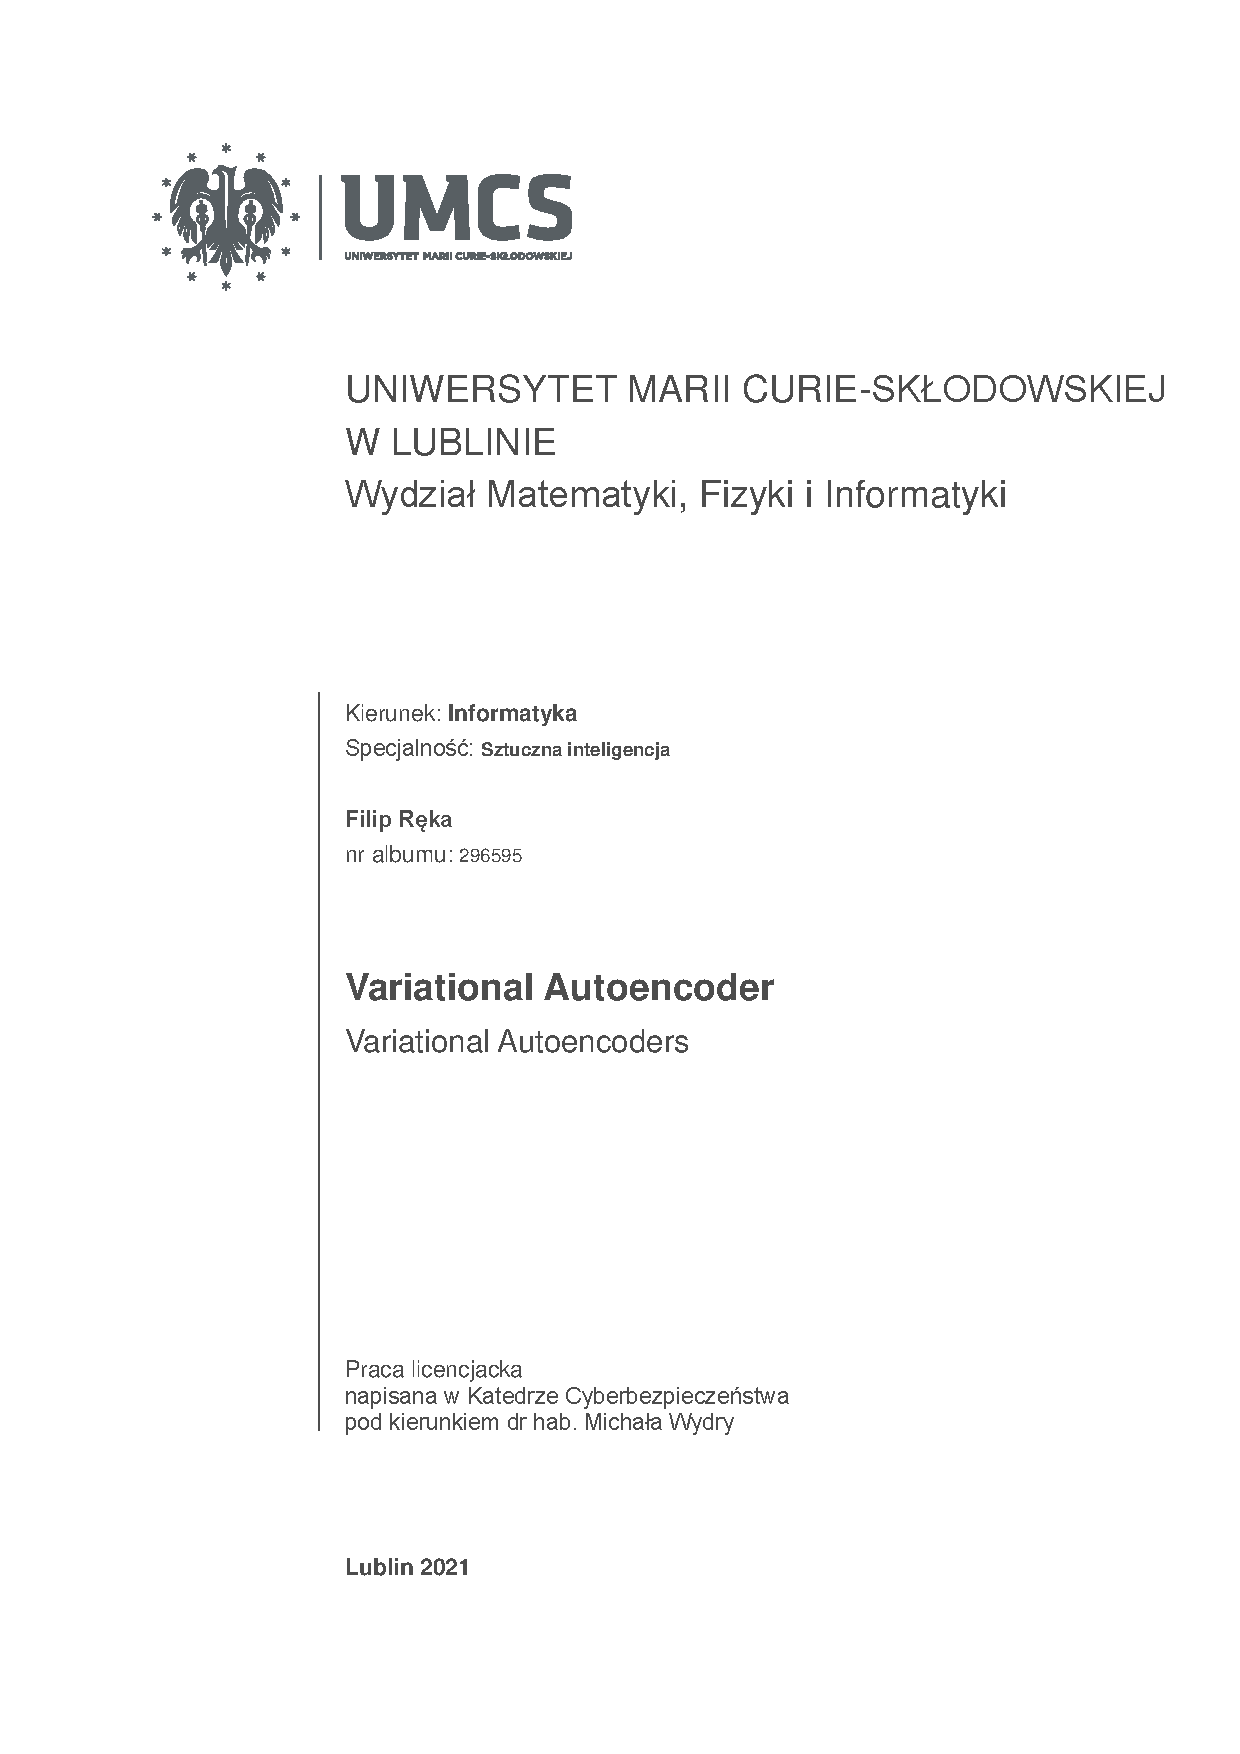
\includepdf{stronatytulowasvg}

%\thispagestyle{empty}

\tableofcontents{}

\chapter*{Wstęp} % z gwiazdką, więc bez numerka...
\addcontentsline{toc}{chapter}{Wstęp} % ...ale w spisie treści ma być
\textbf{Autoenkoder} jest jednym z rodzajów sieci neuronowych, której zadaniem jest nauczenie się zakodowania nie oznaczonych danych. Kod jest kolejnie wykorzystywany do ponownego wygenerowania wejścia sieci. Autoenkoder uczy się reprezentacji zbioru danych do zmiennych ukrytych przez ignorowanie nie istotnych danych.
Wariacyjne autoenkodery są popularnymi modelami generacyjnymi. Zostały zaproponowane przez Diederika P Kingma i Maxa Wellinga w roku 2014.\cite{kingma2014autoencoding} Najczęściej zostają one skategoryzowane do modeli uczenia częściowo nadzorowanego. Znajdują zastosowanie w generacji obrazów, tekstu, muzyki oraz w detekcji anomalii. W przeciwieństwie do tradycyjnych autoenkoderów prezentują pobabilistyczne podejście do generowania zmiennych ukrytych. Swoją popularność zawdzięcza swojej budowie, która jest oparta na sieciach neuronowych oraz możliwości trenowania ich przy pomocy metod gradientowych.
\chapter{Tradycyjny autoenkoder} 
\section{Informacje wstępne}
Autoenkoder jest specyficzną wersją sieci neuronowej składającej się z dwóch części: enkodera, który koduje dane wejściowe oraz dekodera, który na podstawie kodu rekonstruuje wejście.\cite{bank2021autoencoders} Architektura enkodera wymaga aby jego warstwa wyjściowa generująca reprezentacje danych była mniejsza niż warstwa wejściowa. Często zwężenie to jest nazywane \textit{bottle neck}. Model na swoją warstwę wejściową oraz wyjściową dostaję te same dane. Powiedzmy że mamy dane wejściowe $X$ o wymiarze $m$ oraz chcemy je zakodować do wymiaru $n$. Formalnie możemy zapisać:\\
\begin{center}
	Enkoder $E: \mathbb{R}^m \rightarrow \mathbb{R}^n$\\
	Dekoder $D: \mathbb{R}^n \rightarrow \mathbb{R}^m$ \\
	gdzie $n < m$\\
\end{center}
Calem \textit{bottle neck-a} jest skompresowanie wejścia i zachowanie w ukrytych wartościach jak najwięcej informacji. W momencie, kiedy $n = m$ model przekazałby wartości z pierwszej warstwy na ostatnią bez potrzeby kompresji. Celem treningu całego autoenkodera jest zminimalizowanie błędu pomiędzy prawdziwymi danymi wejściowymi, a tymi odkodowanymi ze skompresowanych wartości. W przypadku obrazów funkcją straty może być na przykład błąd średniokwadratowy lub binarna entropia krzyżowa, która powie nam, jak wynik różni się od wejścia. 
 \begin{center}
 		$\mathcal{L}(x, \hat{x}) = \dfrac{1}{m}\displaystyle\sum_{i=0}^{m}(x_i-\hat{x}_i)^2 = \dfrac{1}{m}\displaystyle\sum_{i=0}^{m}(x_i-D(E(x_i)))^2$
 \end{center}

\begin{figure}[h]
	\centering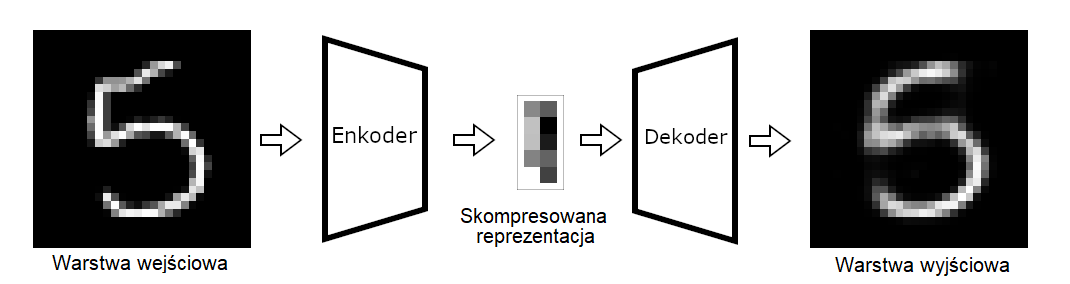
\includegraphics[width=14.5cm]{pictures/autoencoder.png}
	\caption{Schemat budowy autoenkodera.}
\end{figure}
\newpage
\subsection{Zbiór danych MNIST}
Zbiór danych MNIST (\textit{Modified National Institute of Standards and Technology}) jest zbiorem wielu odręcznie pisanych cyfr.\cite{mnist} Znajduje szerokie zastosowanie w nauce i prezentacjach możliwości modeli uczenia maszynowego. W jego skład wchodzi 60,000 obrazów przeznaczonych do treningu modeli oraz 10,000 do testów. Obrazy są czarno-białe i mają wymiary 28 na 28 pikseli.
\begin{figure}[h]
	\centering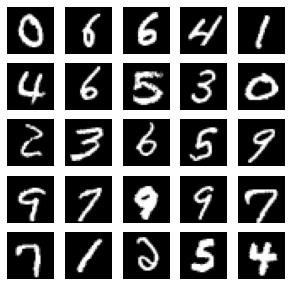
\includegraphics[width=5cm]{pictures/mnist.png}
	\caption{Przykładowe obrazy ze zbioru danych.}
\end{figure}
\newpage
\section{Budowa}
Jak już zostało napisane, autoenkoder składa się z dwóch sieci neuronowych. Enkoder jak i dekoder są w pełni połączonymi sieciami neuronowymi. \\
\begin{figure}[!h]
\centering
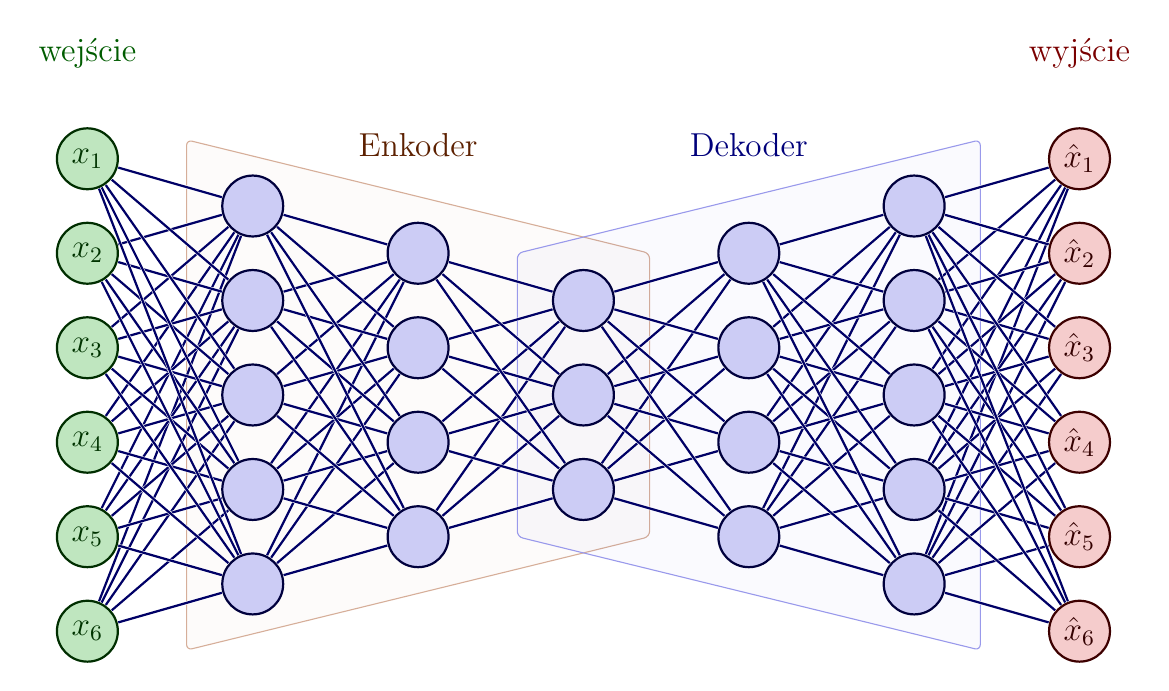
\begin{tikzpicture}[x=2.1cm,y=1.2cm]
	\large
	\readlist\Nnod{6,5,4,3,4,5,6} % array of number of nodes per layer
	
	% TRAPEZIA
	\node[above,align=center,myorange!60!black] at (3,2.4) {Enkoder};
	\node[above,align=center,myblue!60!black] at (5,2.4) {Dekoder};
  	\draw[myorange!40,fill=myorange,fill opacity=0.02,rounded corners=2]
		(1.6,-2.7) --++ (0,5.4) --++ (2.8,-1.2) --++ (0,-3) -- cycle;
	\draw[myblue!40,fill=myblue,fill opacity=0.02,rounded corners=2]
		(6.4,-2.7) --++ (0,5.4) --++ (-2.8,-1.2) --++ (0,-3) -- cycle;
	
	\foreachitem \N \in \Nnod{ % loop over layers
		\def\lay{\Ncnt} % alias of index of current layer
		\pgfmathsetmacro\prev{int(\Ncnt-1)} % number of previous layer
		\message{\lay,}
		\foreach \i [evaluate={\y=\N/2-\i+0.5; \x=\lay; \n=\nstyle;}] in {1,...,\N}{ % loop over nodes
			
			% NODES
			\ifnum \Ncnt = 1
				\node[node \n,outer sep=0.6] (N\lay-\i) at (\x,\y) {$x_\i$};
			\else
				\ifnum \Ncnt = 7
					\node[node \n,outer sep=0.6] (N\lay-\i) at (\x,\y) {$\hat{x}_\i$};
				\else
					\node[node \n,outer sep=0.6] (N\lay-\i) at (\x,\y) {};
				\fi
			\fi
			
			% CONNECTIONS
			\ifnumcomp{\lay}{>}{1}{ % connect to previous layer
				\foreach \j in {1,...,\Nnod[\prev]}{ % loop over nodes in previous layer
					\draw[connect,white,line width=1.2] (N\prev-\j) -- (N\lay-\i);
					\draw[connect] (N\prev-\j) -- (N\lay-\i);
					%\draw[connect] (N\prev-\j.0) -- (N\lay-\i.180); % connect to left
				}
			}{} % else: nothing to connect first layer
			
		}
	}
	
	% LABELS
	\node[above=0.5,align=center,mygreen!60!black] at (N1-1.90) {wejście};
	\node[above=0.5,align=center,myred!60!black] at (N\Nnodlen-1.90) {wyjście};
	
\end{tikzpicture}
\caption{Wizualizacja sieci tworzącej autoenkoder.}
\label{fig:aenetwork}
\end{figure}\\
Obrazek \ref{fig:aenetwork} przedstawia prosty autoenkoder kompresujący wejście siedmiowymiarowe do kodu o długości trzy. Enkoder jak i dekoder mają po dwie warstwy ukryte. Odbicie lustrzane architektury nie jest konieczne aby model działał poprawnie, jednak zwyczajem jest używanie takiej architektury.\\
Hiperparametramy modelu, które możemy ustalić przed jego treningiem to:
\begin{itemize}
	\item Ilość warstw ukrytych - jeśli wiemy, że nasze dane są skomplikowane, dodatkowe warstwy ukryte będą miały pozytywny wpływ na otrzymywane rezultaty, ponieważ większa ilość warstw sprawia, że model jest w stanie nauczyć się bardziej skomplikowanych funkcji.\cite{telgarsky2016benefits, eldan2016power}
	\item Ilość neuronów w poszczególnych warstwach - autoenkoder powinien posiadać w każdej warstwie mniej neuronów niż w poprzedniej. W ten sposób model nie będzie ``oszukiwa" i zostaje zmuszony do reprezentacji jak najlepszej kompresji.
	\item Funkcja straty - najlepszymi funkcjami straty do treningu autoenkodera jest błąd średniokwadratowy lub binarna entropia krzyżowa w przypadku, kiedy dane są w przedziale od 0 do 1.
	\item Rozmiar kodu - jest najistotniejszy parametr dla nas i dla modelu. Dłuższa długość kodu oznacza zachowanie więcej istotnych elementów, a co za tym idzie lepsze odwzorowanie przez dekoder. Z drugiej strony używając, dłuższego wektora zmiennych ukrytych dostajemy gorszą kompresje danych. Długość kodu musimy dobrać w zależności od problemu, który chcemy rozwiązać używając model.
\end{itemize}
\section{Zastosowania}
\subsection{Redukcja wymiaru}
Redukcja wymiaru jest procesem zmniejszenia liczby zmiennych przeznaczonych do analizy, a zarazem zachowanie w nich jak najwięcej istotnych informacji. Powody dla których chcemy zmniejszyć wymiarowość danych to między innymi:
\begin{itemize}
	\item Część zmiennych opisująca dane jest ze sobą nadmiernie skorelowana lub niesie ze sobą cechy, które nie są istotne statystycznie i usunięcie ich nie wpływa na poprawę działania modeli statystycznych lub uczenia maszynowego.
	\item Dane bardzo wysokiego wymiaru są trudne do analizy lub operacje na nich zajmują tak dużo czasu i zasobów że stają się one bezużyteczne. 
	\item Wielowymiarowe dane jest ciężej zwizualizować. Możemy je zredukować do jedno, dwu, lub trzy wymiarowej reprezentacji co pozwoli nam na proste narysowanie wykresu zrozumiałego przez każdego.
\end{itemize}
Autoenkoder nie jest jednym sposobem na redukcję wymiarów. Najbardziej rozpowszechnioną metodą jest \textit{PCA}. 
\subsubsection{Analiza składowych głównych}
Analiza składowych głównych (\textit{ang. Principal Components Analysis, \textbf{PCA}}) służy do wyznaczania jak najmniejszej ilości nowych zmiennych, mówiących jak najwięcej o zbiorze danych. Wielowymiarowe dane koncentrują się w pewnych podprzestrzeniach oryginalniej przestrzeni. Analiza PCA pozwala znaleźć te podprzestrzenie, które są wektorami pełniącymi rolę nowych osi, które je lepiej opisują.\cite{redukcjawymiarow} Używając tej metody ograniczamy się tylko do przekształceń liniowych. Ilość wektorów względem których można zredukować dane jest równa wymiarowi danych. Środkowy obrazek na rysunku \ref{fig:pca} przedstawia właśnie te wektory na przykładzie dwuwymiarowego zbioru punków. Linia względem której spłaszczane są dane jest tą, która minimalizuje odległość do niej od wszystkich punktów. Dolny wykres rysunku \ref{fig:pca} pokazuje już spłaszczone dane do jednego wymiaru. Nowe wektory są wybierane w taki sposób, aby wariancja rzutów poszczególnych obserwacji była jak największa, co gwarantuje nam odwzorowanie jak największej ilości danych. Każdy kolejny wektor zachowuję się w taki sam sposób oraz jest ortonormalny do poprzednich.
\begin{figure}[h!]
	\centering
	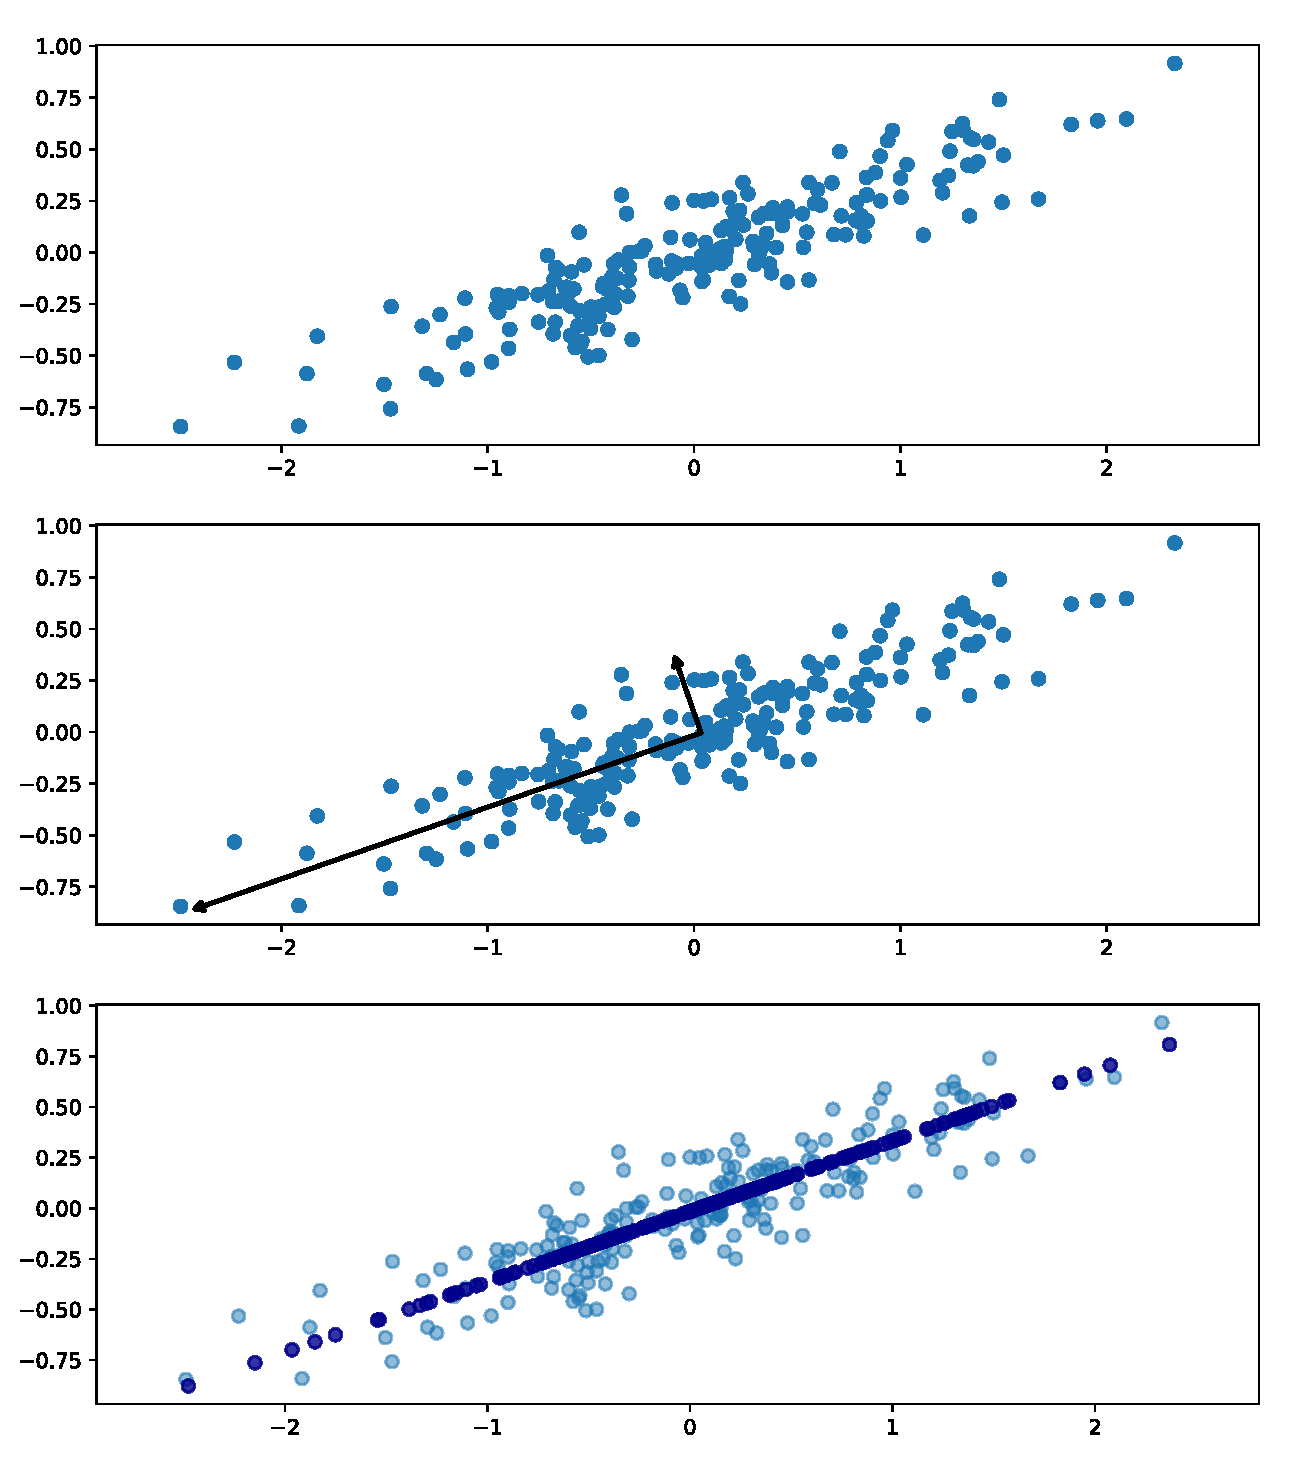
\includegraphics[width=\textwidth]{pca.pdf}
	\caption{Wizualizacja PCA na zbiorze punktów w przestrzeni dwuwymiarowej.}
	\label{fig:pca}
\end{figure}
Wykres \ref{fig:pcacumsum} pokazuje zależność między ilością składników PCA, a procentem wariancji opisywanym przez składniki na podstawie zbioru danych MNIST. Ilość składników mieści się w przedziale od 1 do 784 (28 razy 28 pixeli). Jak można zauważyć dane reprezentowane przez około 80 wartości są w stanie opisać 90\% wariancji danych co jest znaczą redukcją z 784. Przy 400 składnikach osiągamy praktycznie 100\% pokrycia. 
\begin{figure}[h!]
	\centering
	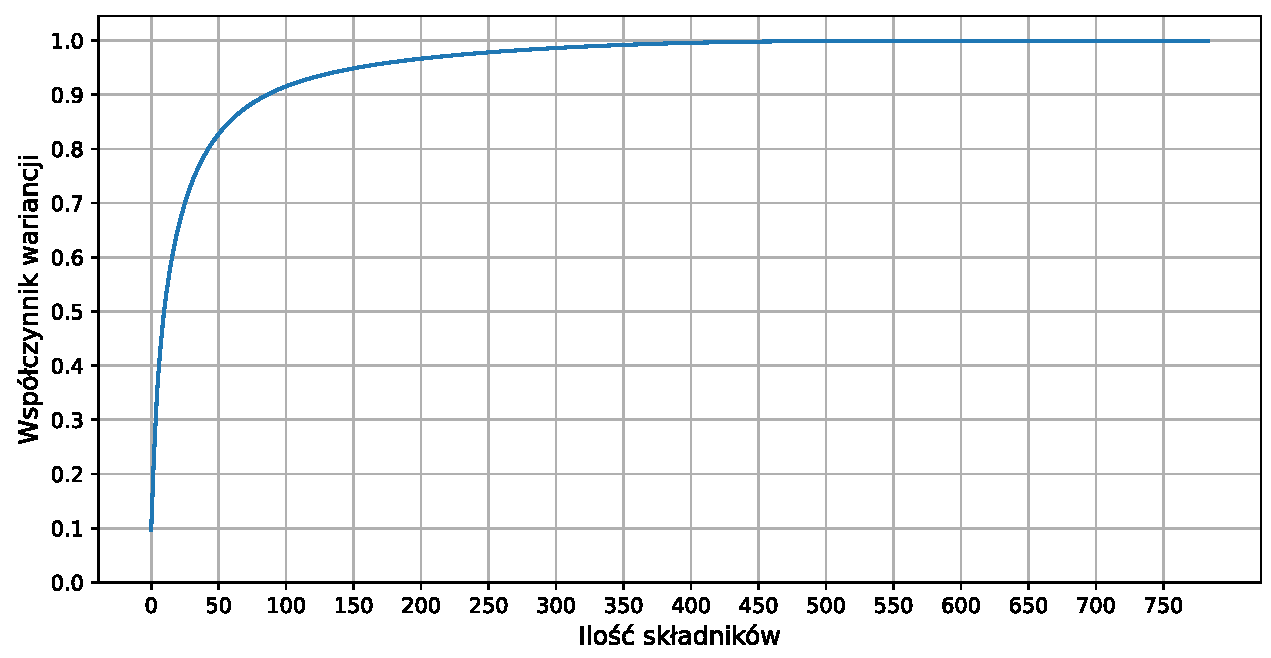
\includegraphics[width=\textwidth]{pcacumsum.pdf}
	\caption{Procent wariancji opisywany przez ilość składników.}
	\label{fig:pcacumsum}
\end{figure}
\subsubsection{Autoenkoder}
\begin{figure}[h!]
	\centering
	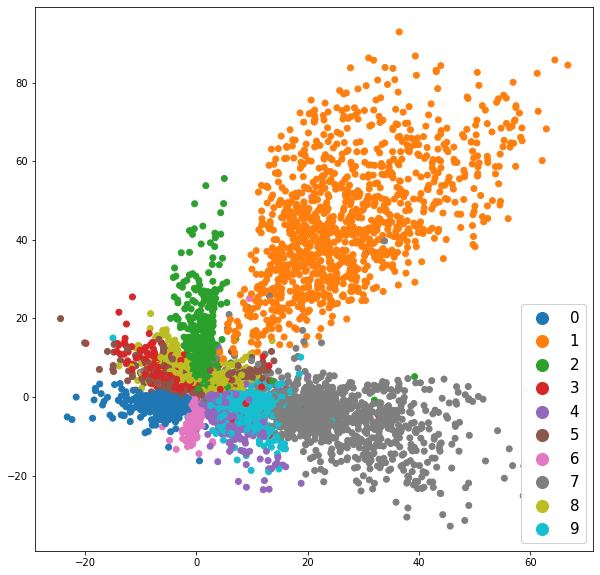
\includegraphics[width=12.5cm]{pictures/aelatentspace.png}
	\caption{Przestrzeń dwuwymiarowej zmiennej ukrytej.}
	\label{fig:latentspaceae}
\end{figure}
\subsection{Odszumianie obrazów}
Model autoenkodera przeznaczony do odszumiania danych, często dostaje swoją nazwę i jest określany mianem DAE \textit{(Denoising autoencoder)}. DAE, tak jak zwykły autoenkoder, próbuje w jak najlepszy sposób skompresować dane, zachowując jak najwięcej istotnych informacji. Najważniejszą różnicą między tymi modelami są dane, które dostają na wejście i wyjście. Obrazy przyjmowane na warstwę wejściową są zaszumione natomiast te z warstwy wyjściowej pochodzą prosto ze zbioru danych.
Powodem dla którego autoenkodery tak dobrze nadają się do odszumiania jest ich umiejętność kompresji danych. Kompresja, której dokonują te modele jest stratna. W przypadku kiedy naszym głównym zadaniem jest jak najlepsze odtworzenie danych wejściowych jest to kłopot, jednak w tym przypadku możemy wykorzystać tą własność na naszą korzyść. Porównując wyjście modelu z danymi bez szumu, zapewniamy, że model nauczy się w jakimś stopniu odtwarzać je poprawnie. Zmuszamy w ten sposób model do ignorowania nieistotnych części naszych danych oraz zapamiętywanie tylko tych, na podstawie których będzie możliwe jak najlepsze odwzorowanie wejścia sieci.
Rysunek \ref{fig:noisedae} pokazuje możliwości modelu na przykładzie zbioru danych MNIST. Do obrazów przeznaczonych do treningu został dodany szum. Zaszumiony obraz powstał przez dodanie do oryginalnego obrazu losowo wybranych wartości z rozkładu Gaussa $\mathcal{N}(0,1)$ przemożonych przez stałą, która w tym przypadku wynosi $0.4$. Następnie obrazy wejściowe zostały skompresowane do kodu o długości pięć, a następnie odkodowane przez dekoder. 
\begin{figure}[h!]
	\centering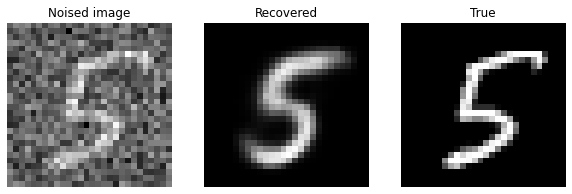
\includegraphics[width=14.5cm]{pictures/noised1.png}
	\caption{Obraz z szumem, odzyskany oraz prawdziwy.}
	\label{fig:noisedae}
\end{figure}

Wadą autoenkoderu przeznaczonego do odszumiania danych jest jego ścisłe powiązanie ze zbiorem danych, na których został wytrenowany. Model z parametrami wytrenowanymi na jednym zbiorze danych nie będzie się nadawał do innego zbioru, z którego danymi będziemy chcieli pracować. Jedynym rozwiązaniem tego problemu jest stworzenie nowego modelu przeznaczonego do użytku na nowych danych. 
\subsection{Uzupełnianie obrazów}
Uzupełnianie obrazów ma na celu wypełnienie brakującej lub zamaskowanej części obszaru. Człowiek bez problemu jest sobie poradzić z tym zadaniem jednak dla komputera nie jest ono oczywiste. Bierze się to z tego, że jest ogromna ilość możliwości wypełnienia nawet niewielkiej brakującej przestrzeni. 
Można wyróżnić dwa główne podejścia wypełniania obrazów:
\begin{itemize}
	\item sieć posiada informację w którym miejscu obrazu jest luka
	\item sieć musi sama się nauczyć, które miejsce obrazu musi wypełnić
\end{itemize}
Rysunek \ref{fig:lukaae} przedstawia drugie podejście. 
\begin{figure}[h]
	\centering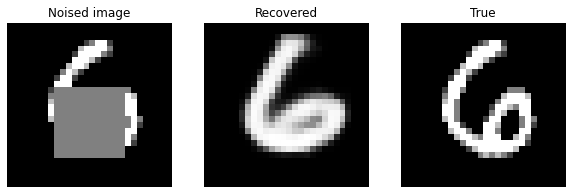
\includegraphics[width=14.5cm]{pictures/completion1.png}
	\caption{Obraz z luką, odzyskany oraz prawdziwy.}
	\label{fig:lukaae}
\end{figure}

\section{Problemy z generacją nowych danych}
Dobrym pytaniem jest czy przy pomocy kodu jesteśmy generować nowe dane bardzo podobne do tych co model otrzymał na wejściu. Wytrenowaliśmy sieć, która jest w stanie ze zmiennych ukrytych odkodować obraz, więc ustawiając wejście dekodera na losowy punkt z przestrzeni zmiennych powinniśmy być w stanie dostać obraz, który jest podobny do tych na których sieć została wytrenowana.
Aby model mógł generować nowe dane muszą zostać spełnione dwa warunki:
\begin{itemize}
	\item Nasza przestrzeń kodu (tzw. zmiennych ukrytych) musi być ciągła co znaczy że dwa punkty znajdujące się obok siebie będą dawać podobne dane jak zostaną odkodowane
	\item Przestrzeń musi być kompletna co znaczy, ze punkty wzięte z dystrybucji muszą dawaj wyniki mające sens
\end{itemize}
Tradycyjna architektura nie zapewnia nam przed treningiem, czy przestrzeń zmiennych ukrytych będzie spełniała te warunki.
Spoglądając na rysunek \ref{fig:latentspaceae} możemy zaobserwować, że przestrzeń zawiera luki. Szczególnie dobrze to widać między klasami oznaczającymi jedynki oraz siódemki. Kolejnym problemem widocznym na tej grafice jest brak separacji między klasami. Niektóre z nich są dobrze odseparowane od siebie, jednak inne całkowicie na siebie nachodzą, jak siódemki z dziewiątkami czy trójki z piątkami. Zadaniem modelu jest jak najlepsze odzwierciedlenie skompresowanych danych, a nie dbanie o to, czy rozkład zmiennych kodu spełnia nasze warunki. Może się tak zdarzyć, że sieć nauczy się akurat takiej dystrybucji, która nam pasuje, ale jest to bardzo mało prawdopodobne. Jeśli chcemy zbudować model generacyjny musimy mieć zagwarantowane, że za każdym razem dostaniemy rozkład spełniający odpowiednie warunki. 
\chapter{Wariacyjny autoenkoder}
\section{Informacje ogóle}
Wariacyjny autoenkoder rozwiązuje problemy generacyjny tradycyjnego modelu. VAE ma na celu skompresowanie danych do określonego wielowymiarowego rozkładu ukrytego, a następnie z próbki z tej dystrybucji, próbuje jak najlepiej zrekonstruować wejście. Najczęściej rozkładami wybieranymi do tego celu są rozkłady normalne. Rozkład normalny jest opisywany przy pomocy dwóch wartości: średnia, która oznaczana jest znakiem $\mu$ oraz odchylenie standardowe oznaczane $\sigma$. Jeśli chcemy dane skompresować do kodu o długości $n$, enkoder wygeneruje dwa wektory $n$-wymiarowe, z którego jeden będzie przechowywał wartości średniej a drugi odchylenia standardowego dla każdego z $n$ rozkładów normalnych.\\
\begin{figure}[h!]
	\centering
	\begin{tikzpicture}
		\node (true) at (-7, 0) {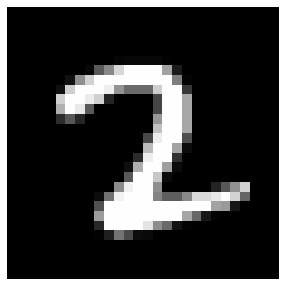
\includegraphics[width=2.5cm]{vaeorg1.png}};
		\draw[thick] (-4.8, 1) -- (-4.8, -1) node[pos=0.5] (enkoderin){} -- (-3.7, -0.6) -- (-3.7, 0.6) node[pos=0.5] (enkoderout){} -- cycle;
		\draw[-latex, thick] (true.east) -- (enkoderin.west);
		\node[scale=0.7](stdv) at (-2.5, 0) {\(\begin{bmatrix}
				0.34 \\ 0.92 \\ \vdots \\ 1.69 \\ 0.38
		\end{bmatrix}\)};
		\node[scale=0.7] (meanv) at (-1.5, 0) {\(\begin{bmatrix}
				0.34 \\ 0.92 \\ \vdots \\ 1.69 \\ 0.38
			\end{bmatrix}\)};
		\draw[-latex, thick](enkoderout.east) -- (stdv.west);
		\node[scale=0.7] (nv) at (0.5, 0) {\(\begin{bmatrix}
				 \mathcal{N}(0.34,0.92)\\ \mathcal{N}(0.34,0.92) \\ \vdots \\ \mathcal{N}(0.34,0.92) \\ \mathcal{N}(0.34,0.92)
			\end{bmatrix}\)};
		\draw[-latex, thick] (meanv.east) -- (nv.west);
		\node[scale=0.7] (sample) at (2.5, 0) {\(\begin{bmatrix}
				0.74 \\ 0.12 \\ \vdots \\ 2.01 \\ 0.13
			\end{bmatrix}\)};
		\draw[-latex, thick] (nv.east) -- (sample.west);
				\draw[thick] (3.7, 0.6) -- (3.7, -0.6) node[pos=0.5] (dekoderin){} -- (4.8, -1) -- (4.8, 1) node[pos=0.5] (dekoderout){} -- cycle;
		\node (recon) at (7, 0) {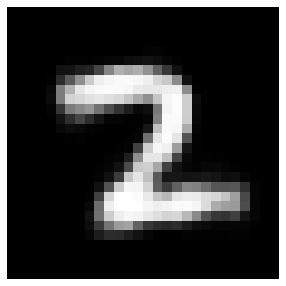
\includegraphics[width=2.5cm]{vaerec1.png}};
		\draw[-latex, thick](sample.east) -- (dekoderin.west);
		\draw[-latex, thick](dekoderout.east) -- (recon.west);
		% Labels
		\node at (-7, -1.5) {wejście};
		\node at (7, -1.5) {wyjście};
		\node at (-2.5, -1.5) {$\sigma$};
		\node at (-1.5, -1.5) {$\mu$};
		\node at (2.5, -1.5) {$z$};
		\node at (0.5, -1.5) {dystrybucje};
		\node at (-4.25, -1.5) {enkoder};
		\node at (4.25, -1.5) {dekoder};

	\end{tikzpicture}
	\caption{Schemat budowy wariacyjnego autoenkodera.}
\end{figure}
\\
 Ograniczając enkoder do nauki wyłącznie tej dystrybucji z której próbkujemy losowo zmienne ukryte z których rekonstruujemy obrazy zapewniamy sobie gładką oraz ciągłą dystrybucje zmiennych losowych. Oczekujemy, że dowolna próbka z przestrzeni zostanie celnie odwzorowana przez dekoder. Dlatego wartości, które sa blisko będą generowały podobne wyjście.\\

\begin{figure}[h!]
	\centering
	\pgfplotsset{
		colormap={whitered}{color(0cm)=(white); color(1cm)=(orange!75!red)}
	}
	\begin{tikzpicture}[
		declare function={mu1=2;},
		declare function={mu2=3;},
		declare function={sigma1=0.5;},
		declare function={sigma2=0.6;},
		declare function={normal(\m,\s)=1/(2*\s*sqrt(pi))*exp(-(x-\m)^2/(2*\s^2));},
		declare function={bivar(\ma,\sa,\mb,\sb)=
			1/(2*pi*\sa*\sb) * exp(-((x-\ma)^2/\sa^2 + (y-\mb)^2/\sb^2))/2;}]
		\begin{axis}[
			colormap name=whitered,
			width=15cm,
			view={45}{55},
			enlargelimits=false,
			grid=major,
			domain=0:5,
			y domain=0:5,
			samples=31,
			xlabel=$x_2$,
			ylabel=$x_1$,
			zlabel={$P$},
			]
			\addplot3 [surf] {bivar(mu1,sigma1,mu2,sigma2)};
			\addplot3 [domain=0:5,samples=31, samples y=0, thick, smooth] (x,5,{normal(mu1,sigma1)});
			\addplot3 [domain=0:5,samples=31, samples y=0, thick, smooth] (0,x,{normal(mu2,sigma2)});
			
			\draw [black!50] (axis cs:-1,0,0) -- (axis cs:4,0,0);
			\draw [black!50] (axis cs:0,-1,0) -- (axis cs:0,4,0);
			
			\node at (axis cs:0,2,0.12) [pin=165:$P(x_1)$] {};
			\node at (axis cs:4,4,0.32) [pin=-15:$P(x_2)$] {};
		\end{axis}
	\end{tikzpicture}
	\caption{Wielowymiarowy rozkład zmiennej.}
\end{figure}
\section{Motywacja statystyczna}
Powiedzmy ze istnieje zmienna ukryta $z$, która generuje obserwację $x$. Posiadamy tylko informację o $x$ i chcemy się dowiedzieć z jakiego $z$ dana obserwacja powstała. Aby tego dokonać powinniśmy policzyć $p(z|x)$. Z twierdzenia Bayesa wiemy że:\\
\begin{center}
	$p(z|x)=\dfrac{p(x|z)p(z)}{p(x)}$
\end{center}
Aby obliczyć rozkład marginalny $p(x)$ musimy policzyć:
\begin{center}
	$p(x) = \displaystyle\int_{z}^{}p(x,z)dz$
\end{center}
Obliczenie tej całki jest bardzo trudne ponieważ $z$ jest często wielowymiarowe i przestrzeń przeszukiwań jest kombinatorycznie zwyczajnie za duża aby korzystać z takich metod jak próbkowanie Monte Carlo łańcuchami Markowa.\textit{citation needed :(} \\

\section{Wnioskowanie wariacyjne}
Rozwiązaniem tego problemu jest próba policzenia rozkładu $q(z|x)$, które będzie jak najlepiej odzwierciedlać $p(z|x)$ i będzie miał rozkład, który będziemy mogli policzyć. 
\subsection{Dywergencji Kullbacka-Leiblera}
Jest to miara określająca rozbieżność między dwoma rozkładami prawdopodobieństwa. Nie można określić jej mianem metryki ponieważ nie jest symetryczna ($D_{KL}(P\|Q)\neq  D_{KL}(Q\|P)$).\\ Naszym celem będzie zminimalizowanie jej.
\begin{center}
	$q^\ast(z|x)=\operatorname*{argmin}_{q(z|x)\in Q}(D_{KL}(q(z|x)\|p(z|x)))$
	\\gdzie $Q$ to rodzina prostych dystrybucji, na przykład rozkładu Gaussa 
\end{center}
Policzmy:
\begin{center}
	$D_{KL}(q(z|x)\|p(z|x))=\mathbb{E}_{z\sim q(z|x)}\log\dfrac{p(z|x)}{q(z|x)} = 
	\displaystyle\int_{z}^{}q(z|x)\log\frac{q(z|x)}{p(z|x)}dz$
\end{center}
	 Natrafiamy na kolejny problem ponieważ nie możemy $p(z|x)$ jednak jesteśmy w stanie to przepisać jako:\\
\begin{center}
	$p(z|x)=\dfrac{p(z,x)}{p(x)}$
\end{center}
Tu jest dużo matmy której nie chce mi się na razie pisać ale tu będzie ELBO (dolna granica dowodów).
\newpage
Wybieramy sobie że nasza funkcja $q(z|x)$ będzie $\mathcal{N}(0, \textit{\textbf{I}})$.
Dywergencja dla dwóch rozkładów normalnych wygląda w następujący sposób. 
\begin{center}
	$\dfrac{1}{2}\left\{\left(\dfrac{\sigma_0}{\sigma_1}\right)^2+\dfrac{(\mu_1 - \mu_0)^2}{\sigma_1^2} - 1 + 2\log\dfrac{\sigma_1}{\sigma_0}\right\}$
\end{center}
Co w naszym przypadku gdzie $\mu_1 = 0$ oraz $\sigma_1=1$ uprości się do:
\begin{center}
	$\dfrac{1}{2}\displaystyle\sum_{m}^{i=1}\sigma_i^2+\mu_i^2-2\log(\sigma_i)-1$
\end{center} 
Jest to pierwsza część naszej funkcji straty. 
\newpage
\section{Budowa tmp}
\begin{figure}[h!]
	\centering
	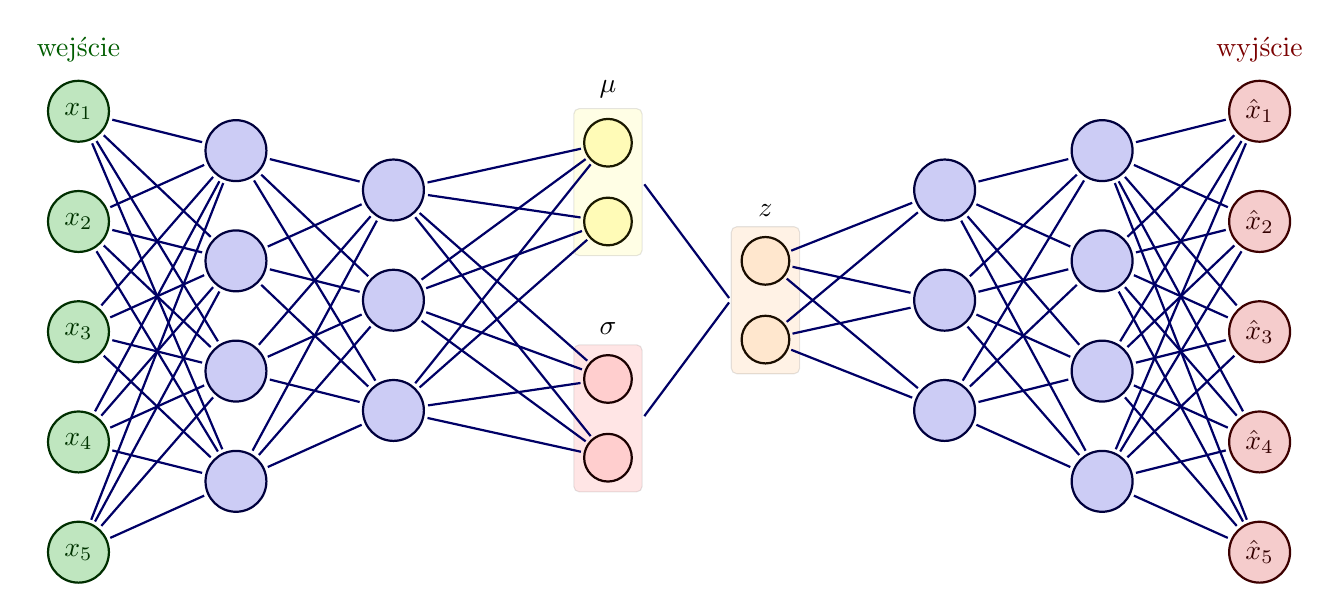
\begin{tikzpicture}[
		shorten >=1pt, shorten <=1pt,
		neuron/.style={circle, draw, minimum size=4ex, thick},
		hidden/.style={node,blue!20!black,draw=myblue!30!black,fill=myblue!20},
		myin/.style={node,green!20!black,draw=mygreen!30!black,fill=mygreen!25},
		myout/.style={node,red!20!black,draw=myred!30!black,fill=myred!20},
		legend/.style={font=\large\bfseries},
		]
		
		% encoder
		\drawEncoder{encoder}{{{,,,,}, {,,,}, {,,}}}
		\denselyConnectNodes{encoder}{{5, 4, 3}}
		
		% decoder
		\begin{scope}[xshift=11cm]
			\drawDecoder{decoder}{{{,,}, {,,,}, {,,,,}}}
			\denselyConnectNodes{decoder}{{3, 4, 5}}
		\end{scope}
		
		% mu, sigma, sample nodes
		\foreach \idx in {1,...,2} {
			\coordinate[neuron, right=2 of encoder-3-2, yshift=\idx cm, fill=yellow, fill opacity=0.2] (mu-\idx);
			\coordinate[neuron, right=2 of encoder-3-2, yshift=-\idx cm, fill=red, fill opacity=0.1] (sigma-\idx);
			\coordinate[neuron, right=4 of encoder-3-2, yshift=\idx cm-1.5cm, fill=orange, fill opacity=0.1] (sample-\idx);
		}
		
		% mu, sigma, sample boxes
		\node [label=$\mu$, fit=(mu-1) (mu-2), draw, fill=yellow, opacity=0.1, rounded corners=2] (mu) {};
		\node [label=$\sigma$, fit=(sigma-1) (sigma-2), draw, fill=red, opacity=0.1, rounded corners=2] (sigma) {};
		\node [label=$z$, fit=(sample-1) (sample-2), draw, fill=orange, opacity=0.1, rounded corners=2] (sample) {};
		
		% mu, sigma, sample connections
		\draw[connect] (mu.east) edge (sample.west) (sigma.east) -- (sample.west);
		\foreach \a in {1,2,3}
		\foreach \b in {1,2} {
			\draw[connect] (encoder-3-\a) -- (mu-\b);
			\draw[connect] (encoder-3-\a) -- (sigma-\b);
			\draw[connect] (sample-\b) -- (decoder-1-\a);
		}
	
		\node[above=0.1 of encoder-1-1,mygreen!60!black] {wejście};
		\node[above=0.1 of decoder-3-1,myred!60!black] {wyjście};
		
	\end{tikzpicture}
\end{figure}
\newpage
\section{Sztuczka reparametryzacyjna}
Model \textit{VAE} po zakodowaniu wejścia dokonuje operacji próbkowania (\textit{sampling}) z dystrybucji na nauczonych parametrach. Przy propagacji do przodu nie jest to problem, jednak podczas propagacji wstecznej jest to nie możliwe. Operacja próbkowania nie jest różniczkowalna co sprawia, że nie możemy policzyć gradientu po którym będziemy schodzić. Sposobem obejścia tego problemu jest zastosowanie sztuczki (\textit{reparameterization trick}). Próbkowanie z dystrybucji $z\sim\mathcal{N}(\mu, \sigma)$ jesteśmy w stanie zapisać jako:
\begin{center}
	$\epsilon\sim\mathcal{N}(0,1)$\\
	$z=\mu+\sigma\bigodot\epsilon$
\end{center} 
Pozornie nic się nie zmieniło, jednak teraz jesteśmy w stanie poprowadzić gradient przez $z$, które jest teraz deterministycznie. W poprzednim przypadku było ono losowe wybierane z dystrybucji. \\
\begin{figure}[h!]
	\centering
	\begin{tikzpicture}
		\node (dc) at (-4,0) {Dekoder};
		\node[shape=circle, draw=black, scale=1.2] (z) at (-4,-2) {$z$};
		\node (q) at (-2.6,-2) {$\sim q(z|x)$};
		\node[shape=diamond, draw=black] (sigma) at (-4,-4) {$\sigma$};
		\node[shape=diamond, draw=black] (mu) at (-6, -4) {$\mu$};
		\node (en) at (-5, -6) {Enkoder};
		
		\path[->] (z) edge node[left] {} (dc);
		\path[->] (mu) edge node[left] {} (z);
		\path[->] (sigma) edge node[left] {} (z);
		\draw[-to](-5, -5.5) -- (-5, -4.5);
		
		\node (dc1) at (4,0) {Dekoder};
		\node[shape=diamond, draw=black] (z1) at (4,-2) {$z$};
		\node (q1) at (6,-2) {$z=\mu+\sigma\bigodot\epsilon$};
		\node[shape=diamond, draw=black] (sigma1) at (4,-4) {$\sigma$};
		\node[shape=diamond, draw=black] (mu1) at (2, -4) {$\mu$};
		\node (en1) at (3, -6) {Enkoder};
		\node[shape=circle, draw=black, scale=1.2] (epsilon) at (6, -4) {$\epsilon$};
		\node (n) at (7.5, -4) {$\sim\mathcal{N}(0,1)$};
		
		\path[->] (z1) edge node[left] {} (dc1);
		\path[->] (mu1) edge node[left] {} (z1);
		\path[->] (sigma1) edge node[left] {} (z1);
		\path[->] (epsilon) edge node[left] {} (z1);
		\draw[-to](3, -5.5) -- (3, -4.5);
		
		\draw[-to](-1.5, -2) -- (2, -2) node[midway, above]{Reparametryzacja};
		
		\node[shape=diamond, draw=black, scale=1.2] (legend-diamond) at (-6, -7) {};
		\node[shape=circle, draw=black, scale=1.4] (legend-circle) at (-6, -8) {}; 
		\node (determin) at (-3, -7) {- węzeł deterministyczny};
		\node (randnode) at (-3.94, -8) {- węzeł losowy};
	\end{tikzpicture}
	\caption{Graficzna reprezentacja reparametryzacji.}
\end{figure}
\chapter{Implementacja}
\section{Tensorflow oraz Keras}
\lipsum[1]\cite{doersch2021tutorial}

\listoftables{} % jeśli są tabele
\addcontentsline{toc}{chapter}{Spis tabel}

\listoffigures{} % jeśli są tabele
\addcontentsline{toc}{chapter}{Spis rysunków}

\bibliographystyle{ieeetr}
\bibliography{./cytowania/cytowania.bib}

\end{document}
